%%%%%%%%%%%%%%%%%%%%% chapter.tex %%%%%%%%%%%%%%%%%%%%%%%%%%%%%%%%%
%
% sample chapter
%
% Use this file as a template for your own input.
%
%%%%%%%%%%%%%%%%%%%%%%%% Springer-Verlag %%%%%%%%%%%%%%%%%%%%%%%%%%
%\motto{Use the template \emph{chapter.tex} to style the various elements of your chapter content.}
\chapter{对话理解与智能质检}
\label{basic} % Always give a unique label
% use \chaptermark{}
% to alter or adjust the chapter heading in the running head
本节首先给出对话理解任务的定义,然后介绍对话理解的主要方法。接下来以智能质检为例,讲述对话理解是怎么落地和实现的。
\section{对话理解}
\subsection{什么是对话理解}
对话理解是指希望计算机跟人一样,具备自然语言理解的能力,从对话内容中挖掘对话意图,理解对话意图,用户情绪识别等。例如,在客服与用户交互的对话中,用户询问“今天的天气如何”,这里就是一个“询问天气”的意图。在实际对话中,
由于自然语言的多义同义问题,语言的词序问题,我们不能只停留在字面理解层面,更需要语义层面的理解。

这里对话可以包含语音对话和文本对话,如果是语音对话,我们一般可以利用语音自动识别技术将语音转为文本。后续我们要讨论的内容是文本的对话理解。
\subsection{技术路线简介}
一般而言,文本的对话理解从技术角度上可以分为两类:文本匹配和文本分类。

\textbf{文本匹配}~~~文本匹配的目标是得到$f(text_1, text_2)$的语义匹配得分,其中$text_1$和$text_2$是输入的文本,$f$是文本匹配模型。传统文本匹配技术主要按照字面上词汇重合度来进行文本匹配,比如传统信息检索中的向量空间模型VSM、BM25等算法。这种基于词汇重合度的匹配算法存在一定的局限性。例如“出租车”和“的士”语义是一致的,但是字面上却完全不匹配。近年来,随着深度学习技术的发展,我们通过多层神经网络对文本语义进行建模,在语义匹配效果上有了很大的提升。

深度学习的模型主要包含Representation-based Match和Interaction-based Match两种,如下图所示。

\begin{figure}[ht]
\centering
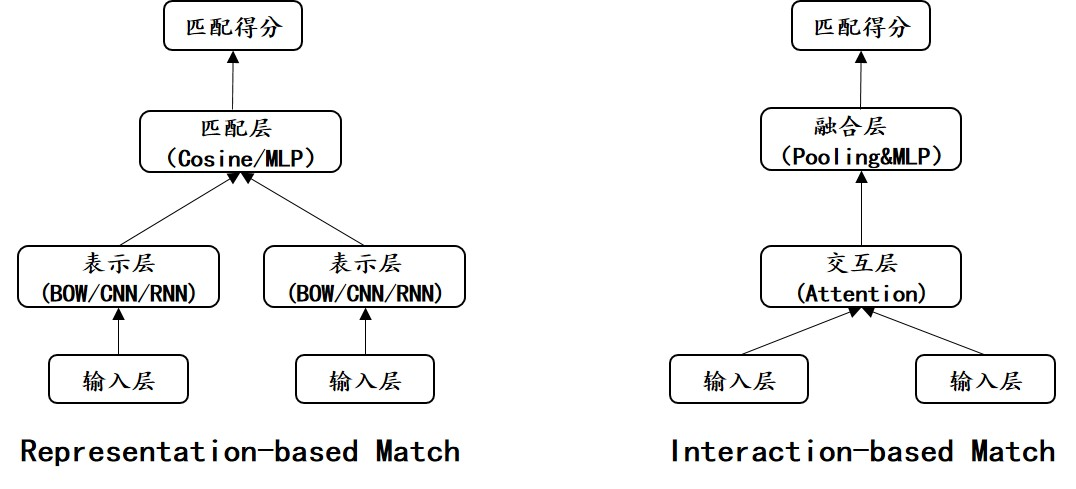
\includegraphics[scale=0.6]{./img/chapter4_b/representation-interaction.jpg}
\caption{Representation-based Match和Interaction-based Match框架图}
\label{fig1}
\end{figure}
输入层一般是将词通过look-up table变成词向量,常见的方法有word2vec, 其后陆续出现了一些文本向量化方法, 如GloVe, FastText, EMLo等,不过word2vec几乎还是最适用的方法之一。词到向量的转化使得词与词之间的语义相似性可以通过向量相似度的方法来度量。为了减少数据稀疏,我们可以加入subword information,即词内的结构信息,中文里面就是字的信息,英文就是字母的信息。

Representation-based Match的核心思想是先将句子转为向量,然后再匹配。怎么获得句子向量呢?最简单的方式有Bag of Words(BOW),句子中词向量求和作为句子向量表示,向量求和可以将不定长的句子转化为定长的向量,但BOW的方式忽略了句子中词序对语义带来的影响。当然,句子向量更高级的获取方式可以使用卷积神经网络(CNN)或者循环神经网络(RNN)来得到。有了句子向量,我们通过匹配层去计算两个句子向量的匹配得分,这里匹配层可以是用余弦距离(Cosine Distance)或者把两个句子向量拼接(concatenation)再经过一个多层感知机(MLP)来实现。经典的方法有Siamese CNN,Siamese LSTM,DSSM,ARC-I等。Representation-based Match的优势是可以离线计算好句子向量的表示,易于建立索引,执行效率高,非常适合文本匹配的粗召回。但其存在的问题是容易丢失语义焦点,词的上下文重要性较难捕捉。

Interaction-based Match则是构造了两个句子之间的语义单元(e.g., term,n-gram,part-of-speech)的交互矩阵,然后再经过一个融合层将细粒度的语义匹配信息合并,较好的把握句子的语义焦点和保留重要的句子间相似信息。主流的方法包含ARC-II,DeepMatch和MatchPyramid等。Interaction-based Match不能离线预处理,需要在线匹配,适合精排序。

\textbf{文本分类}~~~文本分类的目标则是得到${g(text)}$的语义标签,其中$text$是输入的文本,$g$是文本分类模型。文本分类问题需要数据标注其语义标签,在任务型对话中,这个语义标签就是意图。文本分类模型训练好后,我们就可以对新数据进行分类了。具体内容可以参考对话系统的章节。

\section{应用案例:智能质检}
对话理解在智能客服,智能质检有着广泛的应用。下面以智能质检为例,阐述对话理解相关技术是怎么应用的。
\subsection{什么是智能质检}

智能质检使用人工智能算法,分析坐席呼叫场景下人工客服与客户的对话,实现全量质量检查,提高人工客服的服务质量和客户的满意度。
智能质检系统的输入是一通人工客服和客户对话的录音,输出是质检报表,显示该录音在不同质检项的合格情况。质检项的重要性通过质检项的分数来决定。
智能质检无需人工介入,节省质检人力,覆盖率高(100\%),提升质检效率,降低漏检错检率。
\begin{figure}[h]
\centering
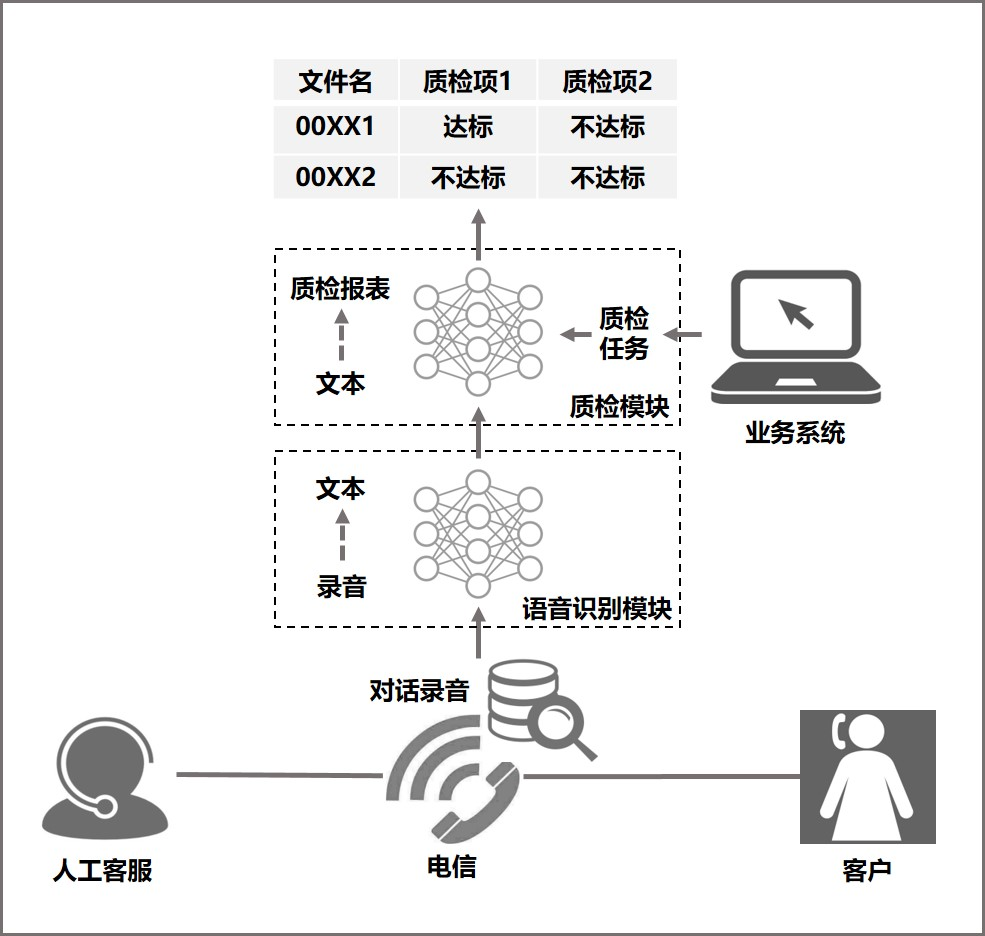
\includegraphics[scale=0.4]{./img/chapter4_b/qic_workflow.jpg}
\caption{智能质检基本流程图}
\label{fig1}
\end{figure}

从智能质检的基本流程图中我们可以发现,对话录音经过语音识别模块之后,我们得到了客户和人工客服之间的对话文本。质检员配置了质检项之后,我们将对话文本输入质检模型,最后得到了质检报表。
\subsection{实现方案与应用状况}
\textbf{实现方案}~~~假设我们定义了质检项要求客服在对话中“核实用户的工作地址”,比如“你的公司地址在哪里”。一种简单的实现方案是通过规则配置“算子+逻辑操作符”或者正则表达式,如果录音文本中满足匹配条件,则命中该质检项。我们可以配置“(公司|工作)\&地址\&(哪|地方)”这样识别出“你的公司地址在哪里”和“您的工作地址在什么地方”这两种说法。这里“公司”就是一个关键词算子,“\&”是一个“与”的逻辑操作符,“|”是一个“或”的逻辑操作符。
这种本质上还是一种基于词汇重合度的匹配算法,适合冷启动,在没有标注数据的情况下就能构建一个简单的质检系统。但它也存在诸多弊端:第一、配置规则需要一定的专业知识,有培训成本;第二、当质检项和表达方式增多时,不同质检项容易出现规则冲突,维护成本高;第三,对于一些比较复杂的质检项,很难通过配置规则进行质检,容易出现漏检和误检的问题。

如果我们有标注数据,就可以使用文本匹配和文本分类的方法。计算$f$(录音文本,质检例句)的语义匹配得分或者$g$(录音文本)的质检项标签。为了减少对数据的依赖和利用大量的无标签数据,一种有效的做法是在BERT(Bidirectional Encoder Representation from Transformers)模型上去fine-tune分类器,BERT用于上层模型的特征提取,作为上层模型的输入,它能够较好的捕捉对话片段的高层语义,兼容少量的漏字情况。我们通过数据驱动的方法让模型越来越聪明,业务方只需要提供标注数据就能进行质检,不需要人工定义规则,模型具有一定的泛化能力。但遇到bad case没有基于规则的方法容易修复,另外需要标注数据积累到一定规模才能发挥模型的优势。

\textbf{应用状况}~~~当前智能质检的应用可以包含离线质检和坐席实时质检。离线质检是指结合语音识别和自然语言处理技术,对海量录音数据进行智能化分析。离线质检可对全量录音质检,质检过程无需人工介入,可以提供内容质检,敏感词识别,语速分析等质检结果。坐席实时质检是指在人工客服和客户对话过程中,提供实时质检能力,辅助人工客服判断客户情绪和实时分析对话过程的信息,及时提醒人工客服从而使客户获得更好的服务。现在智能质检的产品形态包含SaaS云服务和私有化部署。SaaS级产品部署,让中小企业也能够享受智能质检带来的高效与便捷,克服了采购费用高部署周期长的问题。

未来随着多方业务的使用,可以基于联邦学习进行智能质检,在满足数据安全和私隐保护的前提下,通过模型的参数梯度共享,获得了把所有数据放在一起训练的效果,使得不同的业务方合作共赢,建立更准确的数据模型。

